
\setchapterpreamble[u]{\margintoc}
\chapter{\color{gray} Introduction \color{black}}
\labch{intro}

Environmental science has always benefitted from creative approaches for collecting data. However, by itself, a dataset is not enough to make a strong scientific arguement. Data should relate to an appropriate question or hypothesis and should be of sufficient quality that the odds of drawing an incorrect conclusion are low.  For this reason, the scientific process requires that both methods and results be reviewed in a publically-accessible forum--usually a scientific journal. The recent emergence of open-source scientific journals has helped broaden the dissemination of scientific findings to the general public. However, the tools used for scientific data collection often remain sufficiently esoteric that full participation in the scientific process remains out of reach for many interested parties. This textbook focuses on using open-source hardware and software in support of scientifically meaningful environmental data collection projects.  In this context, the term \emph{open-source} refers to equipment, software, and documentation that is available for use by anyone, without any special licensing requirements. The hope is that by publically sharing the systems and processes required to build useful equipment from readily-available components, science itself can also become more accessible.

Some of the projects in the textbook use the built-in sensing capabilities of common electronic platforms, while others use purpose-built digital sensors.  Either way, the intent is to emphasize how sensors can be used for answering relevant questions about environmental systems. We place special emphasis on fields of environmental science and engineering where long-term datasets and/or additional spatial sampling can provide value. Fields and potential applications include:

\begin{itemize}
  \item Hydrology/Climate (water and atmospheric data)
  \item Oceanography (depth, temperature, flow velocity/direction, aquatic chemistry and salinity, waves)
  \item Biology/Ecology (photographic data, water and air quality/temperature, photosynthetically active radiation)
  \item Agriculture (soil moisture, soil temperature, groundwater chemistry)
  \item Geology/Earth Science (seismic monitoring, GPS measurements)
  \item Structural analysis (strain, vibration, corrosion, seismic monitoring)
  \item Environmental Engineering (water/wastewater treatment plant monitoring, monitoring of hydrologic infrastructure such as storage reservoirs, distributed storage values, etc.)
  \item Transportation (traffic counts, programmable signals, vehicle tracking, road noise, autonomous vehicles, pavement integrity, etc.)
\end{itemize}

The primary goal of the textbook is to provide students with enough background that they will be able to plan data collection activities in one or more of these areas \emph{and} be able to justifiy their methodologies with scientific peers. A secondary goal is for students to develop the necessary skills and experience to design, build and use instruments to measure environmental conditions.

\section{\color{gray} Hardware/software choices for this textbook\color{black}}

The ``brain'' of most modern open-source scientific instruments is a \emph{microcontroller}. 
A microcontroller is a device with a processing unit that can run codes and other instructions, and external connections (called \emph{pins}) to transmit electrical inputs and outputs.
The microcontroller is what enables your instrument to receive information from sensors, monitor and regulate its power supply, and communicate for receiving instructions and telemetering data.
Learning to communicate with and control a microcontroller is the first step in building and using environmental sensing instruments.

\subsubsection{Microcontrollers vs. single board computers}

Microcontrollers vary by overall size, power requirements, capabilities to input and output different kinds of electrical signals, onboard communication hardware like WiFi or USB, and the types of code or instructions they accept.
They are distinct from \emph{single board computers} such as Raspberry Pis in that they generally do not incude a robust operating system or the ability to easiy send video directly to a monitor.
While they are relatively constrained in terms of memory and processor power, microcontrollers have the ability to boot and/or wake quickly, reliably perform a pre-defined action such as reading a sensor and/or enabling another device, and then entering a low-power sleep mode until the next action is required. 
This allows a microcontroller to operate automomously for extended periods of time. 


\begin{marginfigure}[-12cm]
	\begin{center}
		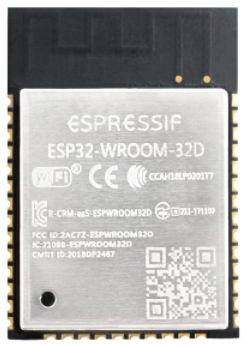
\includegraphics[width=\MFW]{Images/ESP32.png}
		\caption[ESP32 Microcontroller]{This Espressif ESP32 microcontroller module includes a wireless antenna and castellated pads on three sides for making electrical connections.}
		\labfig{ESP32}
	\end{center}
\end{marginfigure}

Microcontroller chips are usually grouped with other components such as power management circuitry, external memory, USB connectors, power and/or reset switches, LEDs, crystal oscillators (used to track time), sensors, and, for those with wireless capabilities, external antennas. 
An example minimal system, an Espressif ESP32 WROOM module mounted next to an antenna and a set of copper pads for making electrical connections, is illustrated in \reffig{ESP32}.
Microcontrollers are usually arranged on a small circuitboard known as a \emph{breakout board} that provides access to the input/output pins on the chip. A good example is the Raspberry Pi Foundation's only true microcontroller, the RPI Pico2040 (\reffig{PICO2040}). (Note that other Raspberry Pi products such as models zero, A, or B include graphics processors and are single board computers). 
A given microcontroller chip may be incorporated into hundreds or thousands of different breakout boards, each of which has slighty different capabilities.
For example a microcontroller board intended to run a small speaker embedded in toy will look very different from one intended to run a robot.
The speaker-based board may just require breaking out just one or two output pins, while the robot controller would require a large number of input/output pins as well as specialized motor control circuitry.

\begin{marginfigure}[-10cm]
	\begin{center}
		\includegraphics[width=\MFW]{Images/PICO2040.png}
		\caption[PICO2040 Microcontroller]{This Raspberry Pi Pico2040 microcontroller module includes a microUSB connector for communicating with a PC in addition to the microcontroller itself, which is the black chip mounted at the center of the board. This board also includes a switch, an on-board LED, power management circuitry, and holes to which header pins can be soldered.}
		\labfig{PICO2040}
	\end{center}
\end{marginfigure}


Systems that use microcontrollers to read a signal from a sensor and then record it to a storage device are referred to as dataloggers.
Dataloggers have been around for many decades, and commerical models have been optimized for low power use and durability.
For many environmental sensing projects, particularly those using sensors with analog voltage or current outputs, a commerical datalogger is an excellent option.
However, commercial dataloggers may not be compatible with digital sensors that require two-way communication to trigger a measurement, and they often cost much more than microcontroller boards.
Furthermore, many modern microcontrollers can also be programmed to communicate wirelessly, opening many new applications for environmental monitoring.
This textbook focuses on using low-cost microcontrollers as datalogging systems for use with both digital and analog sensors.

\subsubsection{Choosing a microcontroller language}
Choosing a microcontroller board that is suitable for a given project can be daunting.
Even within a given microcontroller family, there are many choices to make with respect to both hardware and software.
Until the early 2010s, programming microcontrollers required a specialized set of hardware and software tools.
However, with the release of the Arduino development environment, it became possible to program a variety of microcontrollers using a single framework.
When developing code for an Arduino, the program must be developed using the C programming language.
The human-readable code is then compiled and flashed to the chip, where  it automatically runs when the chip is powered up.
This process results in high performance, low latency programs. 
Perhaps for this reason, Arduino remains one of the most popular open-source microcontroller development frameworks.
However, because there is no easy way to interrupt an Arduino program and check the state of variables, debugging can be challenging.

This textbook focuses on microprocessors that use instructions written in \htmladdnormallink{MicroPython}{https://micropython.org/}, a subset of the \htmladdnormallink{Python}{https://www.python.org} programming language.
MicroPython is a recent invention, and a great improvement for learning about, building and using environmental sensors.
Because MicroPython-based microcontrollers are automatically interactive
\sidenote{\begin{kaobox}[backgroundcolor=\SNcolor,frametitlebackgroundcolor=\SNcolor,frametitle=MicroPython is \texttt{REPL}-ent!]Like Python, MicroPython runs in an interactive session.
	This session goes by the  technical-sounding name \textbf{REPL}, which stands for ``Read-Evaluate-Print-Loop''.
%	, or \emph{REPL}.
	Despite this name, REPL is a very intuitive interface.
	REPL simply means that, in a MicroPython (or Python) session, you type commands, which are then executed, and the results are displayed.
\end{kaobox}}
, they are good platforms for learning to develop and debug codes to collect data from environmental sensors.
MicroPython comes in two main flavors--the standard, officially supported MicroPython release, and CircuitPython, a project supported primarily by Adafruit, a supplier of open source electronics.
CircuitPython is based on MicroPython, but many of the libraries use slightly differnt syntax.
In this textbook, all programs are based on MicroPthon, but it is relatively straightforward to convert CircuitPython code to MicroPython.
For advanced users, this can be helpful becuse it opens the door to using the relatively large number of sensor device drivers that are available in CircuitPython.

Python itself is a powerful and easy to learn language for scientific computing on desktops and laptops.
If you already know some Python, you can apply that knowledge to working with MicroPython-based microcontrollers.
If you're new to Python, then by learning MicroPython you will simultaneously learn how to use Python for many other tasks.
Many of the exercises in this book combine acquiring data from sensors using a microcontroller, and analyzing or plotting those data on a computer, using the same Python coding language.

%\marginnote[3cm]{Note that Python is currently undergoing a transition, from an older version (Python 2.7) to newer Python 3 versions.
%These are mostly similar, but differ in some details such as the syntax of print commands. Because MicroPython is based on Python 3, and because older versions of Python will soon no longer be supported, the codes and instructions in this book will use Python 3.}
%In most cases, Python 2.7 users will need to make only minor adjustments.
\begin{kaobox}[frametitle=Once and future Python]
	Note that Python is currently undergoing a transition, from an older version (Python 2.7) to newer Python 3 versions.
	These are mostly similar, but differ in some details such as the syntax of print commands. Because MicroPython is based on Python 3, and because older versions of Python will soon no longer be supported, the codes and instructions in this book will use Python 3.
\end{kaobox}




%\section{Meet your microcontroller}
%\labsec{microcontrollers}
\subsection{Microcontroller selection}  
Most activities in this textbook have been tested using microchips manufactured by a Chinese company known as Espressif.
Espressif is best known for two families of microcontrollers, the ESP8266 and the more recent ESP32 and its variants, the ESP32-S2 and the ESP32-C3. 
The original ESP8266 microcontroller was designed to be placed in ``smart'' lightbulbs.
\sidenote[][*-8]{\begin{kaobox}[backgroundcolor=\SNcolor,frametitlebackgroundcolor=\SNcolor,frametitle=Lighten up!]See \htmladdnormallink{Tinnkerman's light bulb hacks}{https://tinkerman.cat/post/yet-another-wifi-light-bulb/} for some fun examples in which the ESP8266 microcontroller is reprogrammed in place within a smart light bulb.
Very large scale production for this purpose has made this microcontroller inexpensive, which also makes it a good choice for putting in sensors in often-harsh environments.\end{kaobox}}
Many of the characteristics designed for its intended purpose also make it suitable for environmental sensing instruments.

There are probably hundreds of commercially-available ESP-based breakout boards. 
For this textbook, we focus on using a layout called the Feather form factor, after breakout boards developed by the electronics supplier \emph{Adafruit}.  
Feather-based boards conform to a somewhat standardized breakout board layout, with pins that have unique functions always (or at least usually) located on a particular part of the board.
The standardized layout allows projects built around one microcontroller to be used with different, potentilally more powerful microcontrollers later.
This provides a modest amount of "future-proofing" for the textbook.

The ESP8266 and all the ESP32 chips include wireless communication capabilities that can be used to transmit data remotely through a standard 2.4 Ghz wifi network.
Data posted this way can be accessed online in real time.
Their wireless connectivity makes it possible to program ESP chips directly over the air using a wifi connection and an HTML-based utility known as the WebREPL (micropython.org/webrepl/).  
The WebREPL can be opened in any web browser, so it can be used by PC, Mac, or Linux-based computers.
Files can also be transferred to and from the board using the WebREPL.
This textbook assumes that you have access to a wireless network over which you can communicate with the ESP.
However, for simplicity and because many university networks include enterprise-based security that can make programming difficult, many projects store data directly on flash memory that is present on the ESP chip.
The memory is persistent, so any files you create will remain on the chip even if it loses power. 
Once data collection is complete, files can be transferred off the chip using a wired USB connection. 

Adafruit and other manufacturers have incorporated various versions of the ESP chips and other microcontrollers onto Feather-compatible breakout boards. 
MicroPython developers have gone to great lengths to make code compatible across the ESP-based platforms, so most activities that run on the resource-constrained ESP8266 should work on an ESP32-based chip. 
Most textbook exercises can thus be performed with virtually no code modifications using either of two inexpensive of the Feather boards--the Feather HUZZAH ESP8266 microcontroller or the more recent ESP32-S2-based Feather S2. 
Feather form-factor boards are also available for the Raspberry Pi Pico2040 microcontroller. 
These can be even less expensive than the ESP boards, so they may be a good choice if wireless connectivity is not a priortiy. 
However, price differences are modest, so overall, the Feather S2 may be the best all-around choice for new students. 
\marginnote[1cm]{
	The documents \htmladdnormallink{adafruit-feather-huzzah-esp8266.pdf}{https://cdn-learn.adafruit.com/downloads/pdf/adafruit-feather-huzzah-esp8266.pdf} \htmladdnormallink{adafruit-huzzah-esp8266-breakout.pdf}{https://cdn-learn.adafruit.com/downloads/pdf/adafruit-huzzah-esp8266-breakout.pdf} and \htmladdnormallink{adafruit-esp32-s2-feather.pdf}{https://cdn-learn.adafruit.com/downloads/pdf/adafruit-esp32-s2-feather.pdff} are the best overall resources for information about the Adafruit Huzzah Feather and Breakout versions of the ESP8266/ESP32 microcontrollers.
	Please download the document for your microcontroller for future reference about specifications, pin definitions, voltage tolerances, \etc
}


\subsubsection{Meet your microcontroller}
%\subsubsection{How to use this book}

A close-up view of an ESP-based Feather (\reffig{margin_esp8266}) shows the key features that will prove useful for creating functional environmental sensors.
The core microcontroller is the rectangular component near the bottom.
The zigzag line below it is a built-in WiFi antenna.
At the top is a connector for a microUSB cable, used to communicate with the Feather.
Plugging a USB cable into this connector and into your computer automatically supplies power to the microcontroller.
It also automatically supplies a connection for communicating with the microcontroller.% -- see \refsec{usb_connect} for instructions on how to use USB to communicate with your microcontroller.

\begin{marginfigure}[4cm]
	\begin{center}
		\htmladdnormallink{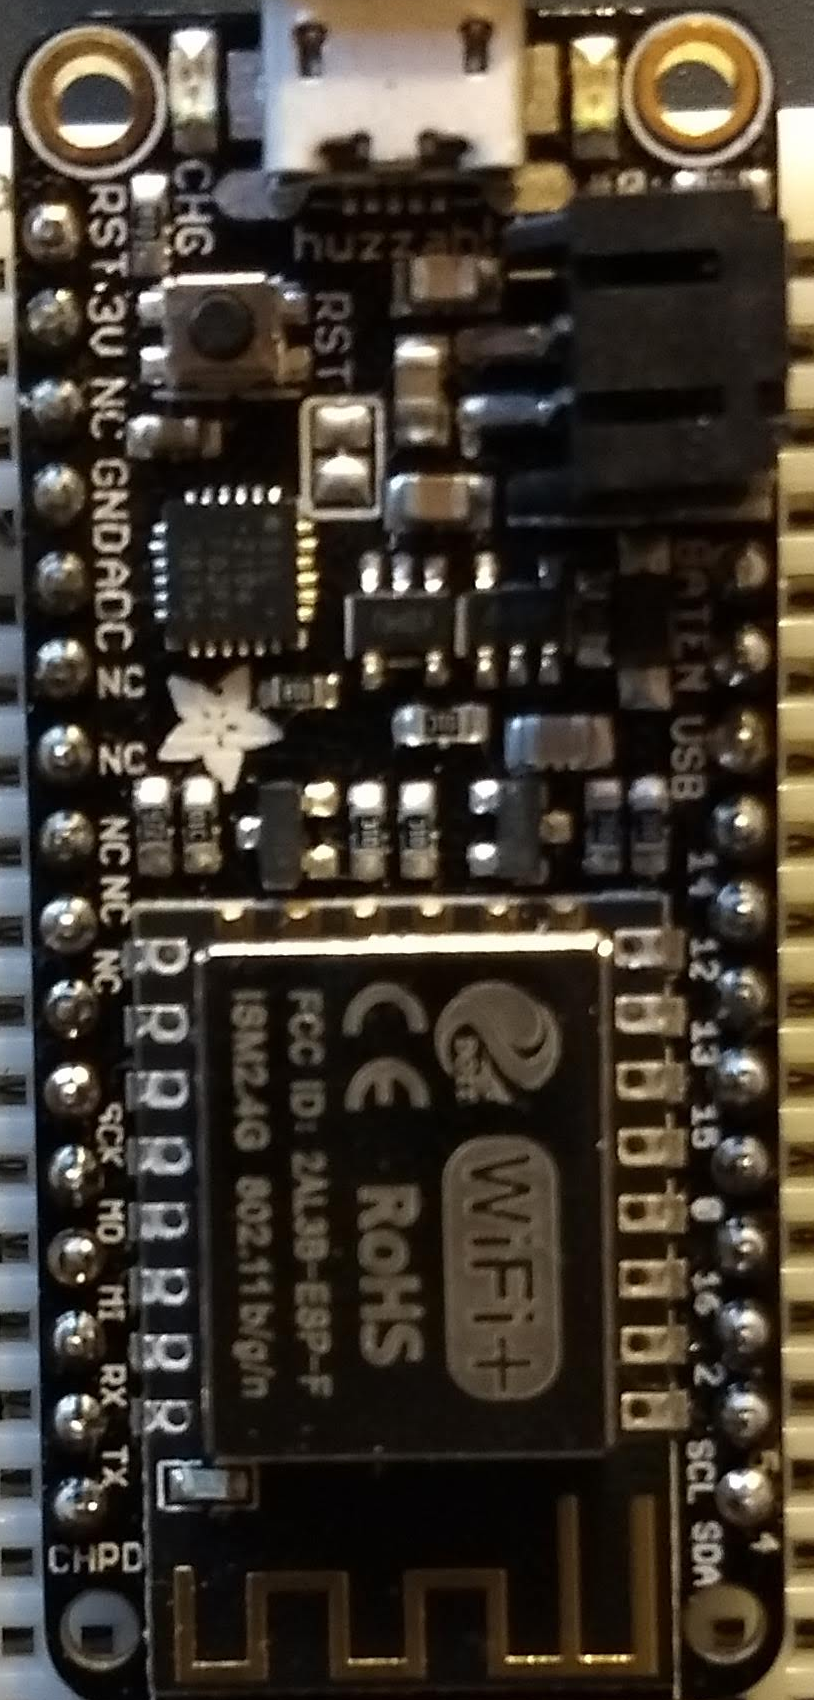
\includegraphics[width=\MFW]{Images/ESP8266feather_top.png}}{https://publicsensors.org/IntroSensors/Images/ESP8266feather_top.png}
		\caption[ESP8266 feather microcontroller]{A ESP8266 Feather microcontroller.}
		\labfig{margin_esp8266}
	\end{center}
\end{marginfigure}

Below and to the left of the USB connector is a button, labelled ``\texttt{RST}''.
This is a reset button, used occasionally to halt a run-away code or reboot a malfunctioning microcontroller (normally we will do this via software, so we rarely need to use the \texttt{RST} button).
At the four corners are holes for mounting screws.
Along the right and left edges are soldered ``pins'', %which are spaced to fit into a breadboard, and
which have different capabilities to transmit electrical signals to and from the microcontroller.
These pins have labels alongside (sometimes a little above or below) that identify the pin, so it can be referred to in MicroPython codes.
We will explain how to use these pins in \refch{first_exercises}.

\begin{kaobox}[frametitle=A flash of insight]
	In these exercises, we assume that your microcontroller already has the basic software needed to run MicroPython. This basic software is called ``firmware'', which must be ``flashed'' onto a microcontroller. The instructions for flashing MicroPython firmware onto your microcontroller are given at the \emph{getting started with MicroPython} tutorials, available for the \htmladdnormallink{ESP8266}{http://docs.micropython.org/en/latest/esp8266/tutorial/intro.html\#intro} or the \htmladdnormallink{ESP32}{https://docs.micropython.org/en/latest/esp32/tutorial/intro.html\#esp32-intro}. If your microcontroller doesn't yet have its firmware, follow the instructions in that tutorial to get ready for the activities in this book. Note that for the ESP32-S2, the best firmware to use is the version for the \htmladdnormallink{TinyS2}{https://micropython.org/download/tinys2/}. 
\end{kaobox}



%\begin{marginfigure}[0cm]
%	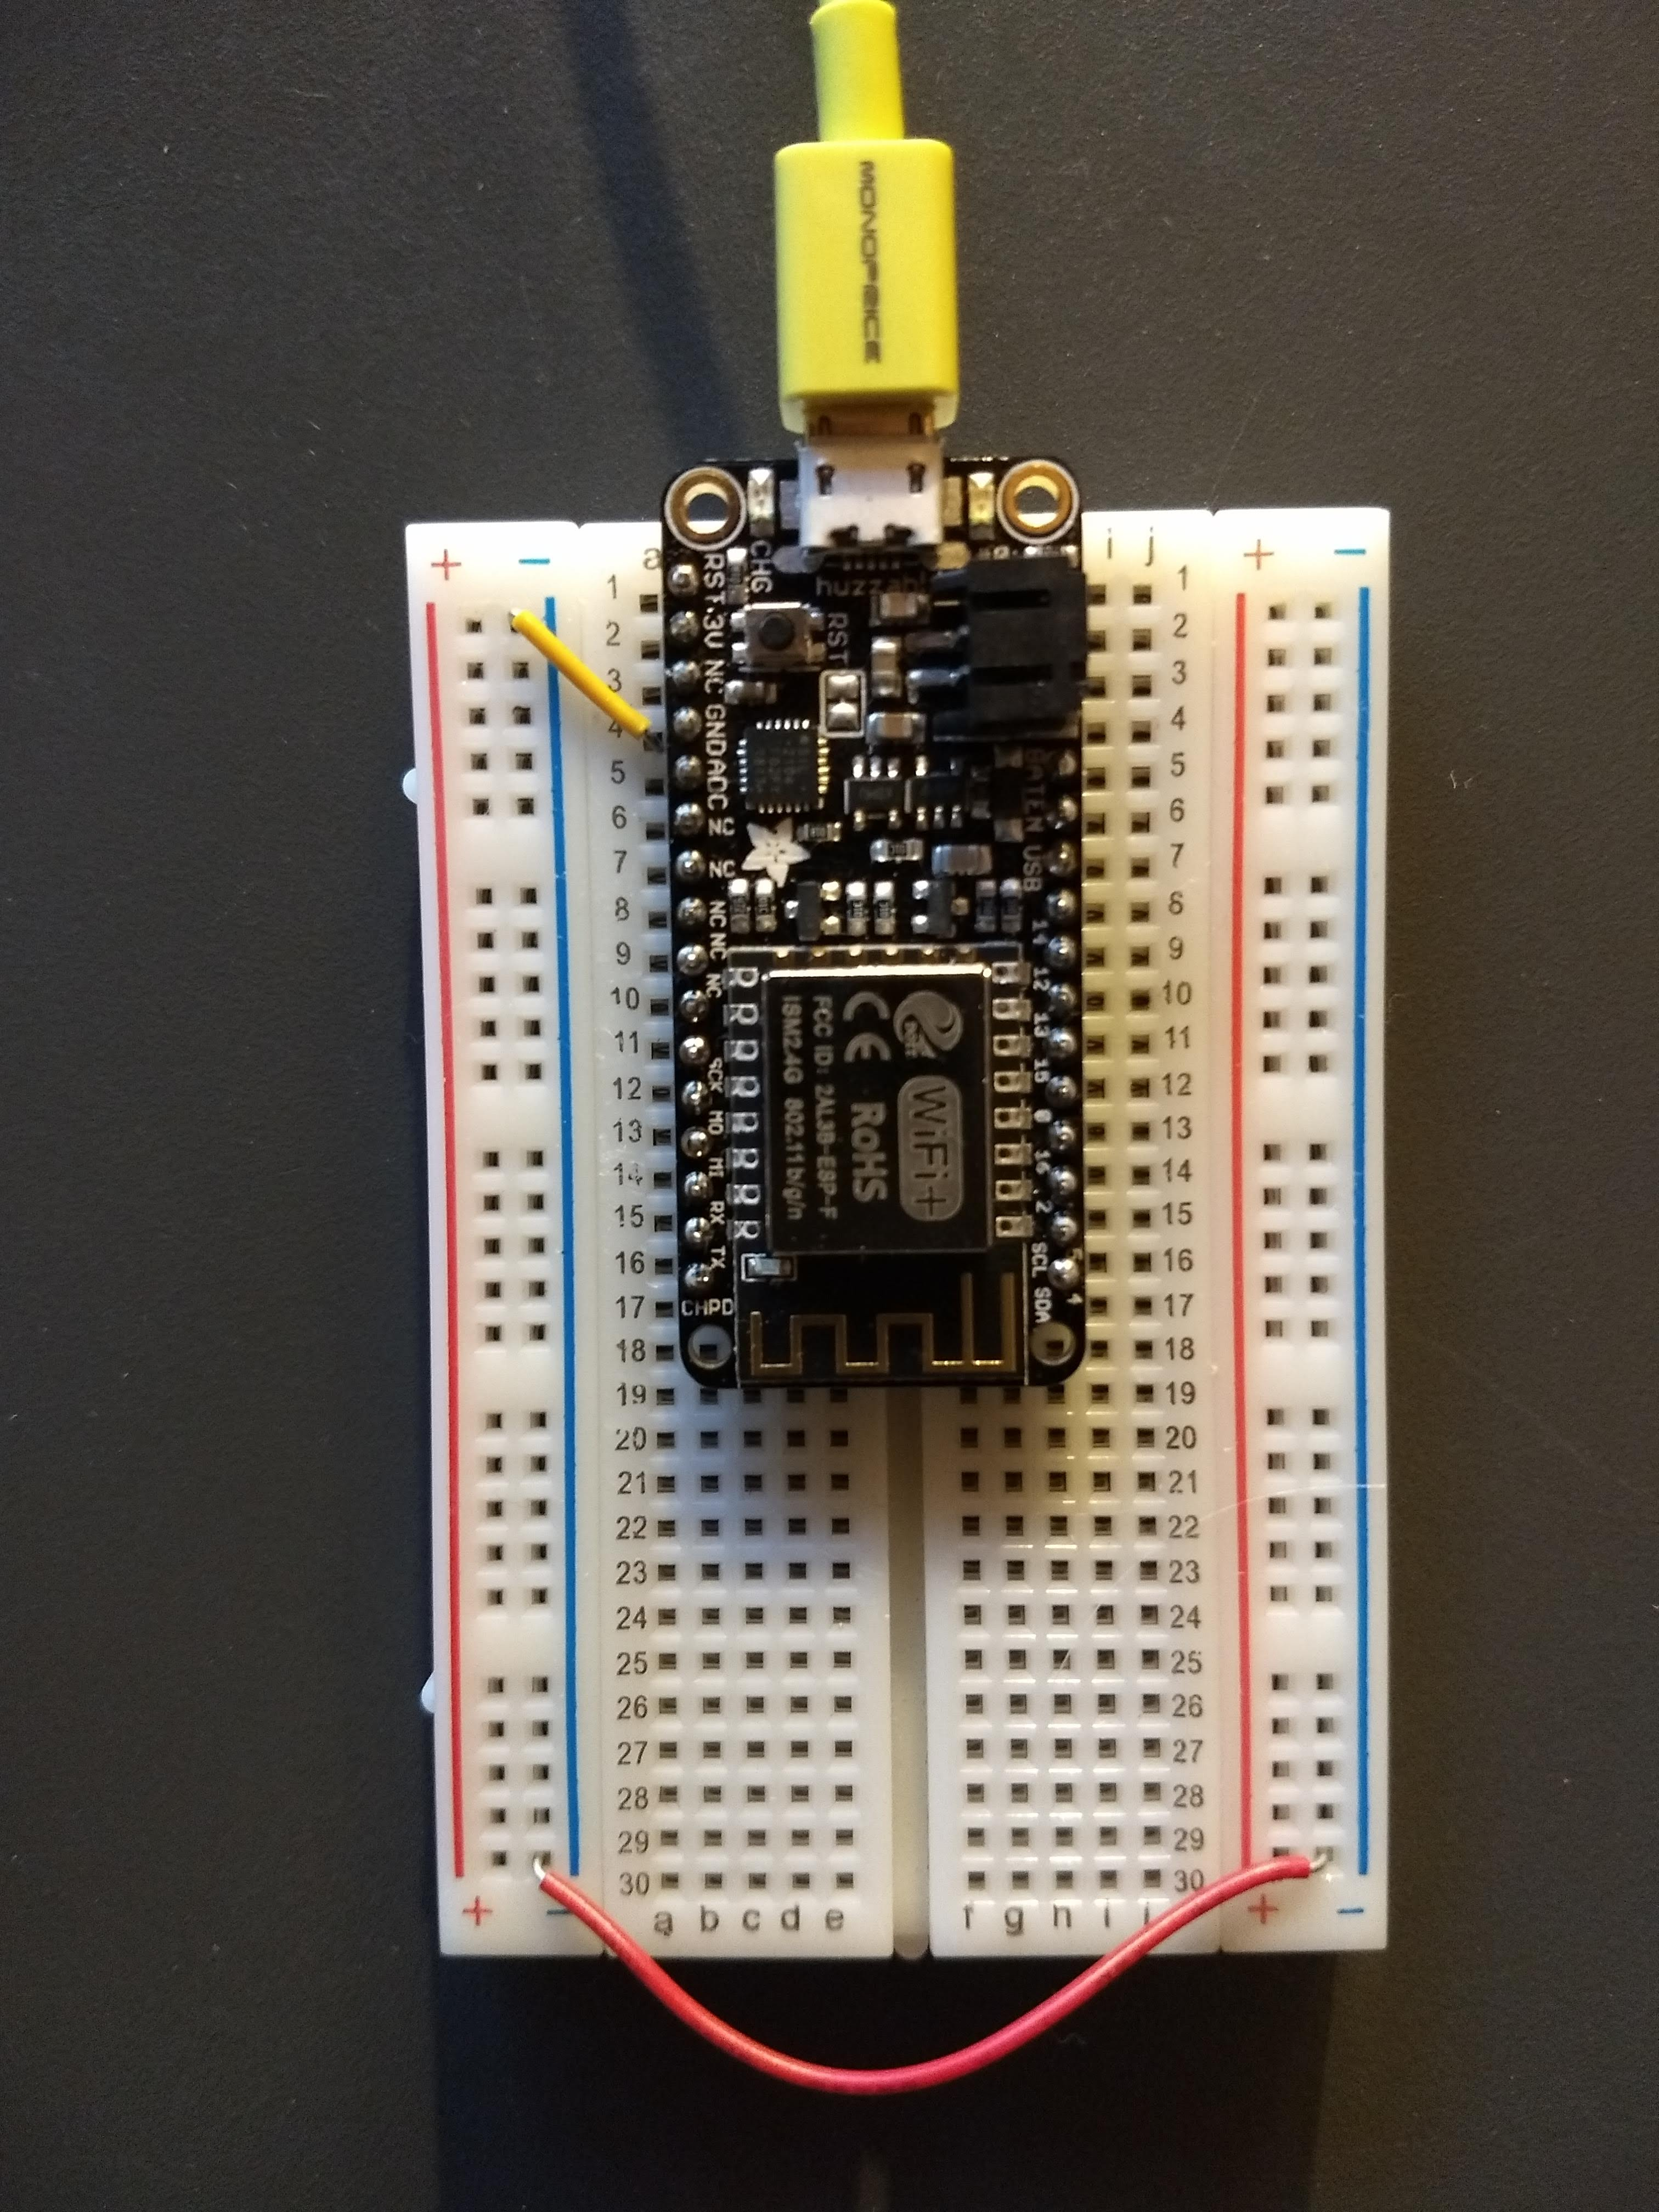
\includegraphics{Images/breadboard_ESP8266feather.jpg}
%	\caption[ESP8266 feather microcontroller on breadboard]{Breadboard with ESP8266 feather.}
%	\labfig{margin_breadboard_esp8266}
%\end{marginfigure}

%%
%%\begin{lstlisting}
%%	\begin{marginfigure}
%%		\includegraphics{Images/IMG_20181205_082817686.jpg}
%%		\caption[ESP8266 feather microcontroller on breadboard, too]{Breadboard with ESP8266 feather, again.}
%%		\labfig{esp8266brd}
%%	\end{marginfigure}
%%\end{lstlisting}
%



\subsection{Other microcontrollers}

We focus here on the ESP8266/ESP32-S2 in Feather form factors because both are officially supported by \htmladdnormallink{MicroPython}{https://http://micropython.org/}, because Adafruit provides good documentation and support, and because they are likely to be available for some time into the future. 
However, many of the exercises in this book can be successfully completed using other microcontrollers, including those mounted on boards that do not comply with the Feather form factor. 
One of the best supported boards is developed by MicroPython.org and is known as a Pyboard.  
While it does not allow for wireless communication, the Pyboard includes several built-in sensors and backup battery management that distinguish it from other MicroPython-based microcontrollers.

Another well-supported microcontroller, Adafruit's HUZZAH ESP8266, is slightly smaller and cheaper than the Feather-based boards, but it requires a special cable for communications rather than a generic microUSB cable.
Many other manufacturers also make microcontroller boards based on the ESP and Pico2040 chips.
Many of these will work in essentially the same way for exercises in this book.
These alternative microcontrollers may require modifying details in the MicroPython codes, such which connections are used for electrical inputs and outputs.
The \htmladdnormallink{MicroPython}{https://http://micropython.org/} website is the best reference if you are considering using alternative microprocessor boards for the activities in this book.

There are also some microcontroller families that work with Adafruit's CircuitPython language but not with MicroPython. CircuitPython's standards make for simpler access the file system on the board, potentially simplifying programming and/or firmware updates. As of 2022, CircuitPython contained a larger number of graphics libraries than does MicroPython, so for projects that require an interface with a screen, CircuitPython-based boards can be a good choice. More information on CircuitPython is available at the \htmladdnormallink{Adafruit}{https://learn.adafruit.com/adafruit-feather-m0-express-designed-for-circuit-python-circuitpython/circuitpython-blinky} site.

\section{\color{gray} Tools needed for working with MicroPython\color{black}}

There are several steps required to set MicroPython up on a new ESP board.  These include 1) ensuring that Python 2.7 or Python 3.4+ are installed on the computer that will be used to set up the microcontroller, 2) ensuring that any USB drivers required by the breakout board are installed on the PC (usually a cp2104 or ch340 driver), 3) downloading and flashing MicroPython to the board, and 4) accessing the board over USB using a terminal program and (optionally) enabling the WebREPL.  These steps are outlined in detail on the  \htmladdnormallink{MicroPython}{https://docs.micropython.org/en/latest/esp8266/esp8266/tutorial/intro.html} website.  

Once a microcontroller is fully setup, it can be connected to the REPL (Read Evaluate Print Loop) using a standard terminal program such as the Chrome-based app \htmladdnormallink{BeagleTerm}{https://chrome.google.com/webstore/detail/beagle-term/gkdofhllgfohlddimiiildbgoggdpoea?hl=en}, the mpfshell terminal, or the Thonny development environment \htmladdnormallink{Thonny development environment}{https://thonny.org/}. To install Thonny, follow this great \htmladdnormallink{tutorial}{https://randomnerdtutorials.com/getting-started-thonny-micropython-python-ide-esp32-esp8266/}. Once Thonny is installed, you should go to Tools, Options, Interpreter, and select “Micropython on a Generic Device”.  You should then be able to power up any Micropython-enabled board through USB and automatically have access to the REPL.  


